%------------------------------------------------------------------------------
\chapter{Auxiliary Information}
\label{sec:app}
% ------------------------------------------------------------------------------

This chapter summarises the event samples used to train and evaluate the models
and auxiliary figures, which are not included in the main part of this thesis.
In Section~\ref{app:samples} the event samples are summarised.
Section~\ref{app:tauid} presents auxiliary figures for the studies of
Chapter~\ref{sec:bdt}. In Section~\ref{app:rnn} additional information on the
RNN-based tau identification from Chapter~\ref{sec:rnn} is given. Finally, in
Section~\ref{app:decay_mode} additional material on the RNN-based decay mode
classification from Chapter~\ref{sec:decaymode} is presented.

\section{Event Samples}
\label{app:samples}

In the following the event samples used for the studies presented in this thesis
are summarised.

\subsection{Samples for BDT- and RNN-based Tau Identification}
\label{app:preprod_taus}
\label{app:preprod_dijets}

\begin{table}[htbp]
  \centering
  {\small
  \begin{tabular}{p{13cm}S[table-format=8.0]}
    \toprule
    Sample & {Events} \\
    \midrule
    \texttt{mc16\_13TeV.425200.Pythia8EvtGen\_A14NNPDF23LO\_Gammatautau\_MassWeight\newline\hspace*{1em}.merge.AOD.e5468\_s2997\_r9064\_r8996} & 19974000 \\
    \bottomrule
  \end{tabular}
  }
  \caption[Signal samples used for BDT- and RNN-based Tau Identification]{Signal
    samples ($\gamma^* \to \tauhad\tauhad$) used for BDT- and RNN-based Tau
    Identification}
  \label{tab:samples_preprod_taus}
\end{table}

\begin{table}[htbp]
  \centering
  {\small
  \begin{tabular}{p{13cm}S[table-format=7.0]}
    \toprule
    Sample & {Events} \\
    \midrule
    \texttt{mc16\_13TeV.361021.Pythia8EvtGen\_A14NNPDF23LO\_jetjet\_JZ1W\newline\hspace*{1em}.merge.AOD.e3569\_s2997\_r9064\_r8996} & 2020000 \\
    \texttt{mc16\_13TeV.361022.Pythia8EvtGen\_A14NNPDF23LO\_jetjet\_JZ2W\newline\hspace*{1em}.merge.AOD.e3668\_s2997\_r9064\_r9078} & 1994000 \\
    \texttt{mc16\_13TeV.361023.Pythia8EvtGen\_A14NNPDF23LO\_jetjet\_JZ3W\newline\hspace*{1em}.merge.AOD.e3668\_s2997\_r9064\_r8996} & 7801500 \\
    \texttt{mc16\_13TeV.361024.Pythia8EvtGen\_A14NNPDF23LO\_jetjet\_JZ4W\newline\hspace*{1em}.merge.AOD.e3668\_s2997\_r9064\_r9078} & 7973500 \\
    \texttt{mc16\_13TeV.361025.Pythia8EvtGen\_A14NNPDF23LO\_jetjet\_JZ5W\newline\hspace*{1em}.merge.AOD.e3668\_s2997\_r9064\_r8996} & 7948500 \\
    \texttt{mc16\_13TeV.361026.Pythia8EvtGen\_A14NNPDF23LO\_jetjet\_JZ6W\newline\hspace*{1em}.merge.AOD.e3569\_s2997\_r9064\_r9078} & 1981000 \\
    \bottomrule
  \end{tabular}
  }
  \caption[Background samples used for BDT- and RNN-based Tau
  Identification]{Background samples (dijet) used for BDT- and RNN-based Tau
    Identification}
  \label{tab:samples_preprod_dijets}
\end{table}

\clearpage
\subsection{Samples for RNN-based Ditau Identification at HL-LHC Conditions}
\label{app:upgrade_samples}

\begin{table}[htbp]
  \centering
  {\small
  \begin{tabular}{p{13cm}S[table-format=6.0]}
    \toprule
    Sample & {Events} \\
    \midrule
    \texttt{mc15\_14TeV.361247.PowhegPythia8EvtGen\_AZNLOCTEQ6L1\_Ztautau\_new\newline\hspace*{1em}.recon.AOD.e4805\_s2987\_s2999\_r8820} & 300000 \\
    \texttt{mc15\_14TeV.301040.PowhegPythia8EvtGen\_AZNLOCTEQ6L1\_DYtautau\_120M180\newline\hspace*{1em}.recon.AOD.e5323\_s2987\_s2999\_r8820} & 150000 \\
    \texttt{mc15\_14TeV.301041.PowhegPythia8EvtGen\_AZNLOCTEQ6L1\_DYtautau\_180M250\newline\hspace*{1em}.recon.AOD.e5323\_s2987\_s2999\_r8820} & 150000 \\
    \texttt{mc15\_14TeV.301042.PowhegPythia8EvtGen\_AZNLOCTEQ6L1\_DYtautau\_250M400\newline\hspace*{1em}.recon.AOD.e5323\_s2987\_s2999\_r8820} & 150000 \\
    \texttt{mc15\_14TeV.301043.PowhegPythia8EvtGen\_AZNLOCTEQ6L1\_DYtautau\_400M600\newline\hspace*{1em}.recon.AOD.e5323\_s2987\_s2999\_r8820} & 147300 \\
    \texttt{mc15\_14TeV.301044.PowhegPythia8EvtGen\_AZNLOCTEQ6L1\_DYtautau\_600M800\newline\hspace*{1em}.recon.AOD.e5323\_s2987\_s2999\_r8820} & 50000 \\
    \texttt{mc15\_14TeV.301045.PowhegPythia8EvtGen\_AZNLOCTEQ6L1\_DYtautau\_800M1000\newline\hspace*{1em}.recon.AOD.e5323\_s2987\_s2999\_r8820} & 50000 \\
    \texttt{mc15\_14TeV.301046.PowhegPythia8EvtGen\_AZNLOCTEQ6L1\_DYtautau\_1000M1250\newline\hspace*{1em}.recon.AOD.e5323\_s2987\_s2999\_r8820} & 50000 \\
    \texttt{mc15\_14TeV.301047.PowhegPythia8EvtGen\_AZNLOCTEQ6L1\_DYtautau\_1250M1500\newline\hspace*{1em}.recon.AOD.e5323\_s2987\_s2999\_r8820} & 50000 \\
    \texttt{mc15\_14TeV.301048.PowhegPythia8EvtGen\_AZNLOCTEQ6L1\_DYtautau\_1500M1750\newline\hspace*{1em}.recon.AOD.e5323\_s2987\_s2999\_r8820} & 49900 \\
    \texttt{mc15\_14TeV.301049.PowhegPythia8EvtGen\_AZNLOCTEQ6L1\_DYtautau\_1750M2000\newline\hspace*{1em}.recon.AOD.e5323\_s2987\_s2999\_r8820} & 50000 \\
    \texttt{mc15\_14TeV.301050.PowhegPythia8EvtGen\_AZNLOCTEQ6L1\_DYtautau\_2000M2250\newline\hspace*{1em}.recon.AOD.e5323\_s2987\_s2999\_r8820} & 50000 \\
    \texttt{mc15\_14TeV.301051.PowhegPythia8EvtGen\_AZNLOCTEQ6L1\_DYtautau\_2250M2500\newline\hspace*{1em}.recon.AOD.e5323\_s2987\_s2999\_r8820} & 49900 \\
    \texttt{mc15\_14TeV.301052.PowhegPythia8EvtGen\_AZNLOCTEQ6L1\_DYtautau\_2500M2750\newline\hspace*{1em}.recon.AOD.e5323\_s2987\_s2999\_r8820} & 50000 \\
    \texttt{mc15\_14TeV.301053.PowhegPythia8EvtGen\_AZNLOCTEQ6L1\_DYtautau\_2750M3000\newline\hspace*{1em}.recon.AOD.e5323\_s2987\_s2999\_r8820} & 50000 \\
    \texttt{mc15\_14TeV.301054.PowhegPythia8EvtGen\_AZNLOCTEQ6L1\_DYtautau\_3000M3500\newline\hspace*{1em}.recon.AOD.e5323\_s2987\_s2999\_r8820} & 50000 \\
    \texttt{mc15\_14TeV.301055.PowhegPythia8EvtGen\_AZNLOCTEQ6L1\_DYtautau\_3500M4000\newline\hspace*{1em}.recon.AOD.e5323\_s2987\_s2999\_r8820} & 50000 \\
    \texttt{mc15\_14TeV.301056.PowhegPythia8EvtGen\_AZNLOCTEQ6L1\_DYtautau\_4000M4500\newline\hspace*{1em}.recon.AOD.e5323\_s2987\_s2999\_r8820} & 50000 \\
    \texttt{mc15\_14TeV.301057.PowhegPythia8EvtGen\_AZNLOCTEQ6L1\_DYtautau\_4500M5000\newline\hspace*{1em}.recon.AOD.e5323\_s2987\_s2999\_r8820} & 50000 \\
    \texttt{mc15\_14TeV.301058.PowhegPythia8EvtGen\_AZNLOCTEQ6L1\_DYtautau\_5000M\newline\hspace*{1em}.recon.AOD.e5323\_s2987\_s2999\_r8820} & 49900 \\
    \bottomrule
  \end{tabular}
  }
  \caption[Signal samples for the Phase-II upgrade of the ATLAS detector]{Signal
    samples ($Z / \gamma^* \to \tau\tau$) for the Phase-II upgrade of the ATLAS
    detector with the Extended ITk-layout.}
  \label{tab:samples_upgrade_tau}
\end{table}

\begin{table}[htbp]
  \centering
  {\small
  \begin{tabular}{p{13cm}S[table-format=6.0]}
    \toprule
    Sample & {Events} \\
    \midrule
    \texttt{mc15\_14TeV.147910.Pythia8\_AU2CT10\_jetjet\_JZ0W\newline\hspace*{1em}.recon.AOD.e2403\_s2987\_s2999\_r8820} & 999500 \\
    \texttt{mc15\_14TeV.147911.Pythia8\_AU2CT10\_jetjet\_JZ1W\newline\hspace*{1em}.recon.AOD.e2403\_s2987\_s2999\_r8820} & 962300 \\
    \texttt{mc15\_14TeV.147912.Pythia8\_AU2CT10\_jetjet\_JZ2W\newline\hspace*{1em}.recon.AOD.e2403\_s2987\_s2999\_r8820} & 999500 \\
    \bottomrule
  \end{tabular}
  }
  \caption[Background samples for the Phase-II upgrade of the ATLAS
  detector]{Background samples (dijet) for the Phase-II upgrade of the ATLAS
    detector with the Extended ITk-layout.}
  \label{tab:samples_upgrade_dijet}
\end{table}


\FloatBarrier
\subsection{Samples for RNN-based Decay Mode Classification}
\label{app:mc16a_taus}

\begin{table}[htbp]
  \centering
  {\small
  \begin{tabular}{p{13cm}S[table-format=8.0]}
    \toprule
    Sample & {Events} \\
    \midrule
    \texttt{mc16\_13TeV.425200.Pythia8EvtGen\_A14NNPDF23LO\_Gammatautau\_MassWeight\newline\hspace*{1em}.merge.AOD.e5468\_s3126\_r9364\_r9315} & 29998000 \\
    \bottomrule
  \end{tabular}
  }
  \caption[Samples used for the RNN-based decay mode classification]{Samples
    used for the RNN-based decay mode classification.}
  \label{tab:samples_mc16a_taus}
\end{table}

\clearpage
\section{Tau Identification using Boosted Decision Trees}
\label{app:tauid}
\subsection{Discriminating Variables}
\label{app:tauid_vars}

\FloatBarrier
\subsubsection{1-prong}
\begin{figure}[htbp]
  \begin{subfigure}{0.5\textwidth}
    \centering
    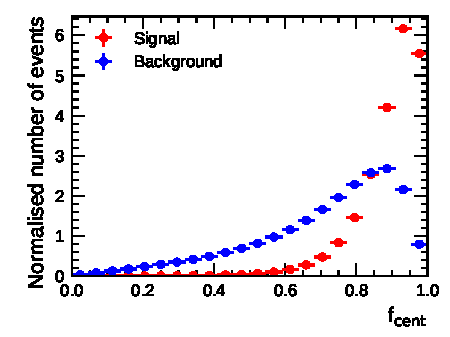
\includegraphics{./figures/baseline_bdt_vars/1p/centFrac.pdf}
  \end{subfigure}%
  \begin{subfigure}{0.5\textwidth}
    \centering
    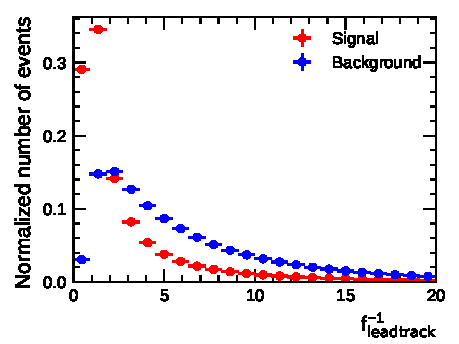
\includegraphics{./figures/baseline_bdt_vars/1p/etOverPtLeadTrk.pdf}
  \end{subfigure}
  \begin{subfigure}{0.5\textwidth}
    \centering
    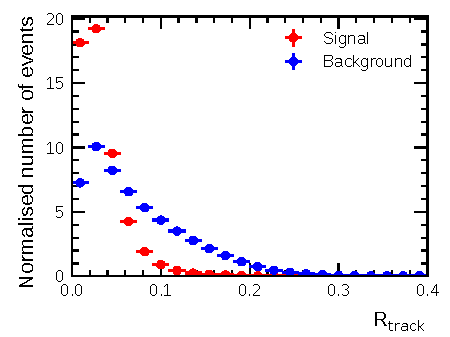
\includegraphics{./figures/baseline_bdt_vars/1p/innerTrkAvgDist_fixed.pdf}
  \end{subfigure}%
  \begin{subfigure}{0.5\textwidth}
    \centering
    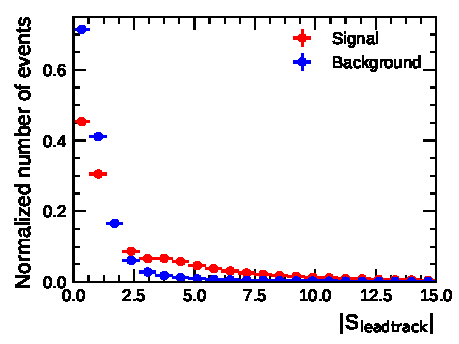
\includegraphics{./figures/baseline_bdt_vars/1p/absipSigLeadTrk.pdf}
  \end{subfigure}
  \begin{subfigure}{0.5\textwidth}
    \centering
    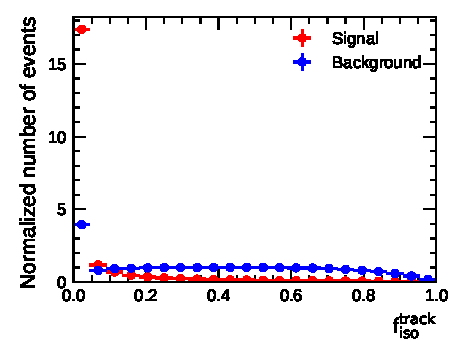
\includegraphics{./figures/baseline_bdt_vars/1p/SumPtTrkFrac.pdf}
  \end{subfigure}%
  \begin{subfigure}{0.5\textwidth}
    \centering
    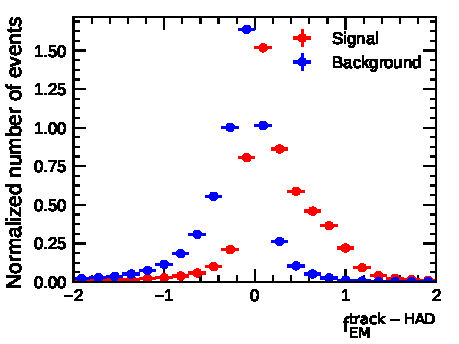
\includegraphics{./figures/baseline_bdt_vars/1p/ChPiEMEOverCaloEME.pdf}
  \end{subfigure}
  \caption[Distributions of variables used for 1-prong tau
  identification]{Distributions of variables used for 1-prong tau
    identification.}
  \label{fig:bdt_vars_1p_overlays}
\end{figure}

\begin{figure}[htbp]\ContinuedFloat
  \begin{subfigure}{0.5\textwidth}
    \centering
    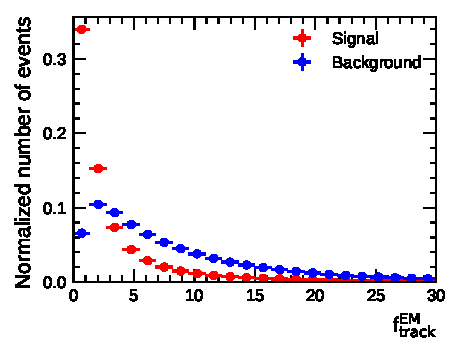
\includegraphics{./figures/baseline_bdt_vars/1p/EMPOverTrkSysP.pdf}
  \end{subfigure}%
  \begin{subfigure}{0.5\textwidth}
    \centering
    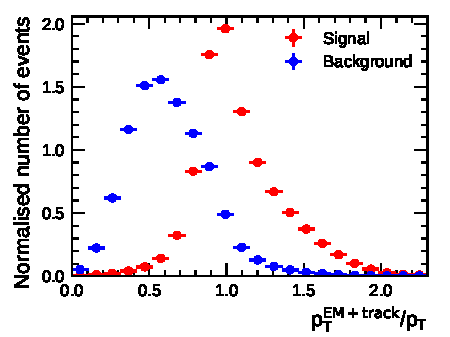
\includegraphics{./figures/baseline_bdt_vars/1p/ptRatioEflowApprox.pdf}
  \end{subfigure}
  \begin{subfigure}{0.5\textwidth}
    \centering
    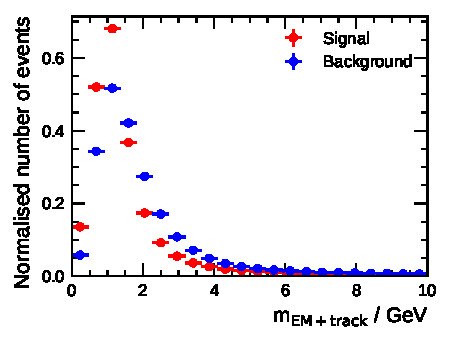
\includegraphics{./figures/baseline_bdt_vars/1p/mEflowApprox.pdf}
  \end{subfigure}
  \caption[]{Distributions of variables used for 1-prong tau identification.}
\end{figure}

\clearpage
\subsubsection{3-prong}

\begin{figure}[htbp]
  \begin{subfigure}{0.5\textwidth}
    \centering
    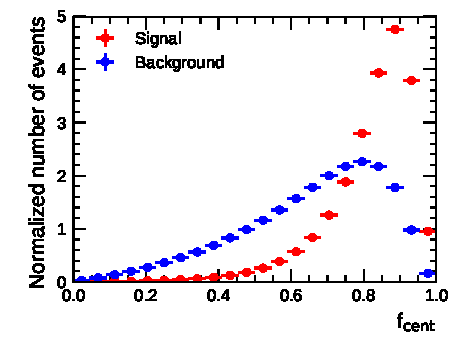
\includegraphics{./figures/baseline_bdt_vars/3p/centFrac.pdf}
  \end{subfigure}%
  \begin{subfigure}{0.5\textwidth}
    \centering
    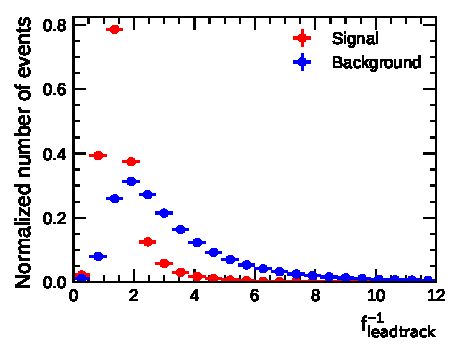
\includegraphics{./figures/baseline_bdt_vars/3p/etOverPtLeadTrk.pdf}
  \end{subfigure}
  \begin{subfigure}{0.5\textwidth}
    \centering
    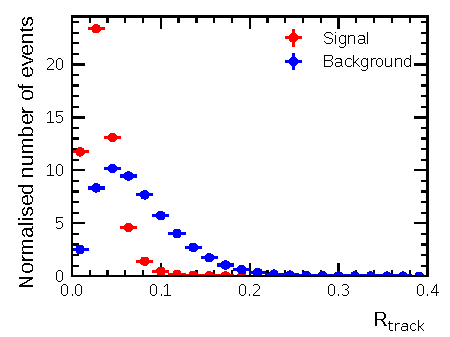
\includegraphics{./figures/baseline_bdt_vars/3p/innerTrkAvgDist_fixed.pdf}
  \end{subfigure}%
  \begin{subfigure}{0.5\textwidth}
    \centering
    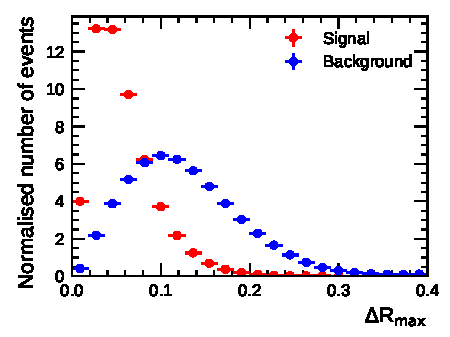
\includegraphics{./figures/baseline_bdt_vars/3p/dRmax.pdf}
  \end{subfigure}
  \begin{subfigure}{0.5\textwidth}
    \centering
    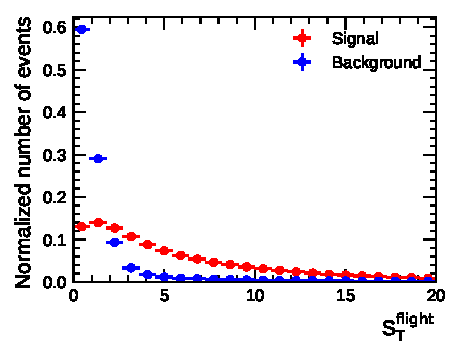
\includegraphics{./figures/baseline_bdt_vars/3p/trFlightPathSig.pdf}
  \end{subfigure}%
  \begin{subfigure}{0.5\textwidth}
    \centering
    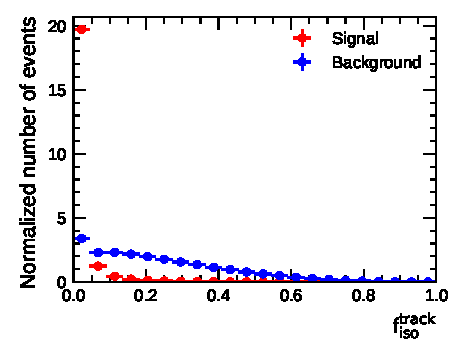
\includegraphics{./figures/baseline_bdt_vars/3p/SumPtTrkFrac.pdf}
  \end{subfigure}%
  \caption[Distributions of variables used for 3-prong tau
  identification]{Distributions of variables used for 3-prong tau
    identification.}
  \label{fig:bdt_vars_3p_overlays}
\end{figure}

\begin{figure}[htbp]\ContinuedFloat
  \begin{subfigure}{0.5\textwidth}
    \centering
    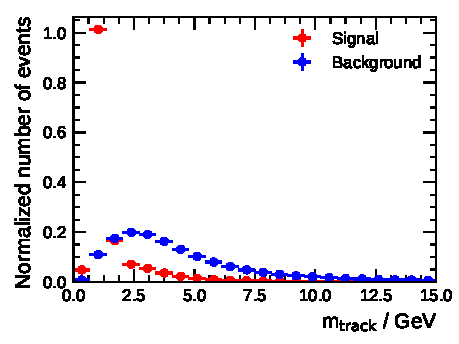
\includegraphics{./figures/baseline_bdt_vars/3p/massTrkSys.pdf}
  \end{subfigure}%
  \begin{subfigure}{0.5\textwidth}
    \centering
    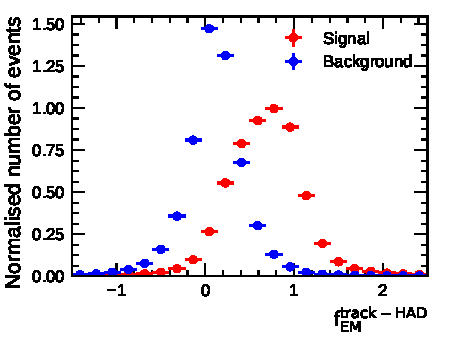
\includegraphics{./figures/baseline_bdt_vars/3p/ChPiEMEOverCaloEME.pdf}
  \end{subfigure}
  \begin{subfigure}{0.5\textwidth}
    \centering
    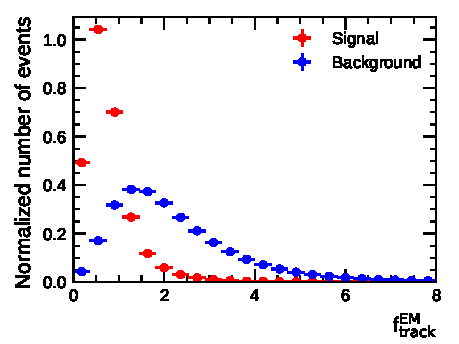
\includegraphics{./figures/baseline_bdt_vars/3p/EMPOverTrkSysP.pdf}
  \end{subfigure}%
  \begin{subfigure}{0.5\textwidth}
    \centering
    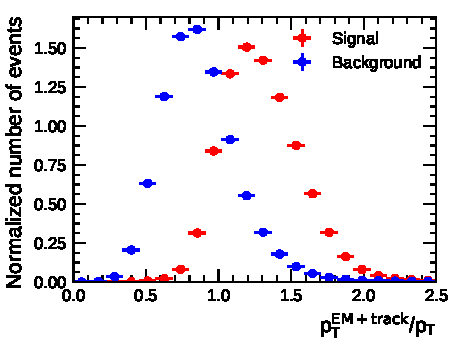
\includegraphics{./figures/baseline_bdt_vars/3p/ptRatioEflowApprox.pdf}
  \end{subfigure}
  \begin{subfigure}{0.5\textwidth}
    \centering
    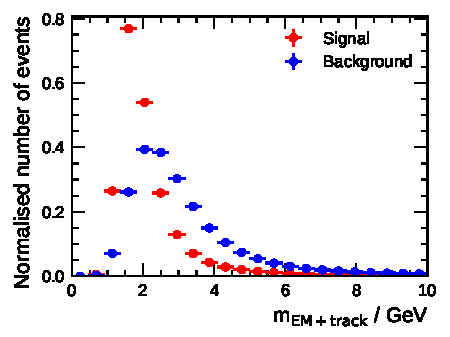
\includegraphics{./figures/baseline_bdt_vars/3p/mEflowApprox.pdf}
  \end{subfigure}
  \caption[]{Distributions of variables used for 3-prong tau identification.}
\end{figure}

\FloatBarrier
\subsection{TMVA-BDT Configurations}
\label{app:tmva_config}

\noindent\textbf{Common for all configurations:}\\[0.3em]
\begin{tabular}{ll}
  \texttt{NegWeightTreatment} & \texttt{IgnoreNegWeightsInTraining} \\
  \texttt{PruneMethod} & \texttt{NoPruning} \\
  \texttt{SeparationType} & \texttt{GiniIndex} \\
  \texttt{UseYesNoLeaf} & \texttt{False} \\
  \texttt{nCuts} & 200
\end{tabular}

\vspace*{1em}

\noindent\textbf{Previous configuration:}\\[0.3em]
\begin{tabular}{ll}
  \texttt{BoostType} & \texttt{AdaBoost} \\
  \texttt{AdaBoostBeta} & 0.2 \\
  \texttt{NTrees} & 100 \\
  \texttt{MaxDepth} & 8 \\
  \texttt{MinNodeSize} & 0.1 \\
\end{tabular}

\vspace*{1em}

\noindent
\begin{minipage}[t]{0.5\textwidth}
\noindent\textbf{1-prong (BDT A):}\\[0.3em]
\begin{tabular}{ll}
  \texttt{BoostType} & \texttt{Grad} \\
  \texttt{Shrinkage} & 0.05 \\
  \texttt{NTrees} & 800 \\
  \texttt{MaxDepth} & 16 \\
  \texttt{MinNodeSize} & 0.01 \\
\end{tabular}

\vspace*{1em}

\noindent\textbf{1-prong (BDT B):}\\[0.3em]
\begin{tabular}{ll}
  \texttt{BoostType} & \texttt{Grad} \\
  \texttt{Shrinkage} & 0.1 \\
  \texttt{NTrees} & 400 \\
  \texttt{UseBaggedBoost} & \texttt{True} \\
  \texttt{BaggedSampleFraction} & 0.5 \\
  \texttt{MaxDepth} & 8 \\
  \texttt{MinNodeSize} & 0.1 \\
\end{tabular}
\end{minipage}%
\begin{minipage}[t]{0.5\textwidth}
\noindent\textbf{3-prong (BDT A):}\\[0.3em]
\begin{tabular}{ll}
  \texttt{BoostType} & \texttt{Grad} \\
  \texttt{Shrinkage} & 0.1 \\
  \texttt{NTrees} & 800 \\
  \texttt{MaxDepth} & 16 \\
  \texttt{MinNodeSize} & 0.01 \\
\end{tabular}

\vspace*{1em}

\noindent\textbf{3-prong (BDT B):}\\[0.3em]
\begin{tabular}{ll}
  \texttt{BoostType} & \texttt{Grad} \\
  \texttt{Shrinkage} & 0.4 \\
  \texttt{NTrees} & 800 \\
  \texttt{MaxDepth} & 6 \\
  \texttt{MinNodeSize} & 0.1 \\
\end{tabular}
\end{minipage}%


\subsection{Variable Transformations}
\label{app:variable_transforms}

\begin{table}[htb]
  \centering
  {\def\arraystretch{1.35}\small
    \begin{tabular}{ll}
  \toprule
  Variable & Transformation \\
  \midrule
  \smash{$f_\text{cent}$} & \smash{$\min(x, 1)$} \\
  \smash{$f_\text{leadtrack}^{-1}$} & \smash{$\log(\max(0.1, x))$} \\
  \smash{$R_\text{track}$} & -- \\
  \smash{$\Delta R_\text{max}$} & -- \\
  \smash{$| S_\text{leadtrack} |$} & \smash{$\min(x, 30)$} \\
  \smash{$S_\text{T}^\text{flight}$} & \smash{$\log(\max(0.01, x))$} \\
  \bottomrule
\end{tabular}\hspace*{2em}
\begin{tabular}{ll}
  \toprule
  Variable & Transformation \\
  \midrule
  \smash{$f_\text{iso}^\text{track}$} & \smash{$\log\left(x + 10^{-4}\right)$} \\
  \smash{$f_\text{EM}^\text{track-HAD}$} & \smash{$\max(-4, \min(x, 5))$} \\
  \smash{$f_\text{track}^\text{EM}$} & \smash{$\log\left(\max\left(10^{-3}, x\right)\right)$} \\
  \smash{$p_\text{T}^\text{EM+track} / p_\text{T}$} & \smash{$\min(x, 4)$} \\
  \smash{$m_\text{EM+track}$} & \smash{$\log\left(\max(140, x / \si{\MeV})\right)$} \\
  \smash{$m_\text{track}$} & \smash{$\log\left(\max(140, x / \si{MeV})\right)$} \\
  \bottomrule
\end{tabular}


%%% Local Variables:
%%% mode: latex
%%% TeX-master: "../mythesis"
%%% End:

  }
  \caption[Transformations applied to input the variables of the BDT-based tau
  identification]{Transformations applied to the input variables of the
    BDT-based tau identification.}
\end{table}

\clearpage
\subsection{Hyperparameter Optimisation (3-prong)}
\label{app:grid_search_3p}

\noindent
\begin{minipage}{\textwidth}
  \captionsetup{type=figure}
  \begin{subfigure}[t]{0.48\textwidth}
    \centering
    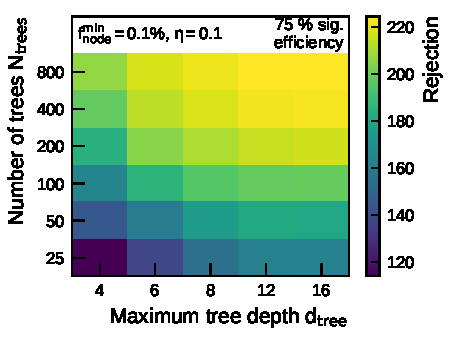
\includegraphics{./figures/bdt_perf/gridsearch_3p/scan_MaxDepth_NTrees.pdf}
  \end{subfigure}\hfill
  \begin{subfigure}[t]{0.48\textwidth}
    \centering
    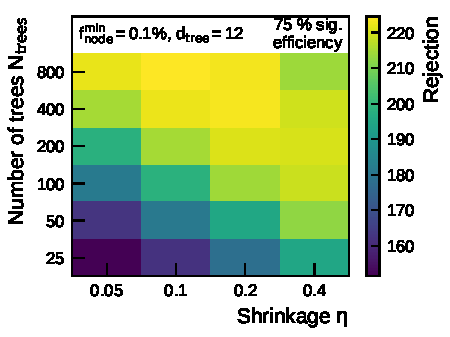
\includegraphics{./figures/bdt_perf/gridsearch_3p/scan_Shrinkage_NTrees.pdf}
  \end{subfigure}
  \begin{subfigure}[t]{0.48\textwidth}
    \centering
    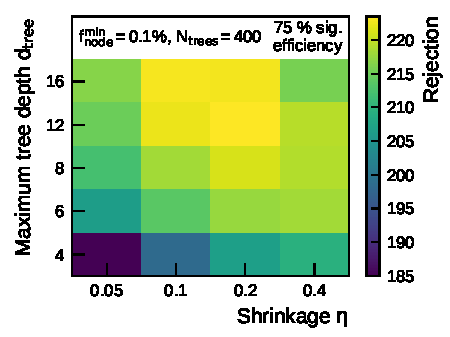
\includegraphics{./figures/bdt_perf/gridsearch_3p/scan_Shrinkage_MaxDepth.pdf}
  \end{subfigure}\hfill
  \begin{subfigure}[t]{0.48\textwidth}
    \centering
    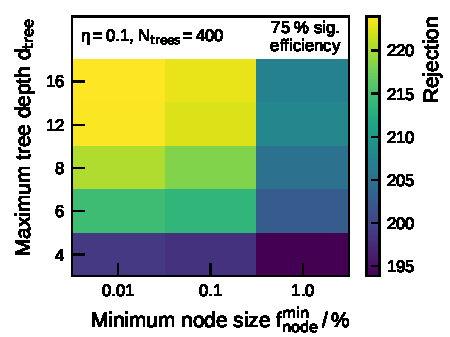
\includegraphics{./figures/bdt_perf/gridsearch_3p/scan_MinNodeSize_MaxDepth.pdf}
  \end{subfigure}
  \caption[Background rejection as a function of BDT hyperparameters
  (3-prong)]{Background rejection of the 3-prong BDT at \SI{45}{\percent} signal
    efficiency as a function of BDT hyperparameters. No bagged boosting is used.
    The rejection is calculated using the testing sample.}
  \label{fig:hyperparameter_scan_3p}
\end{minipage}

\FloatBarrier
\subsection{BDT Score Distributions (3-prong)}
\label{app:bdt_stuff}

\noindent
\begin{minipage}{\textwidth}
  \captionsetup{type=figure}
  \begin{subfigure}[t]{0.48\textwidth}
    \centering
    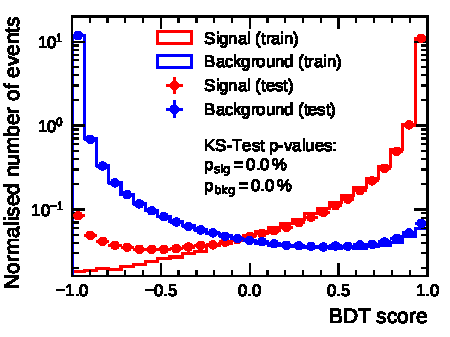
\includegraphics{./figures/bdt_perf/scores/grid_3p0317.pdf}
    \subcaption{BDT A}
  \end{subfigure}\hfill
  \begin{subfigure}[t]{0.48\textwidth}
    \centering
    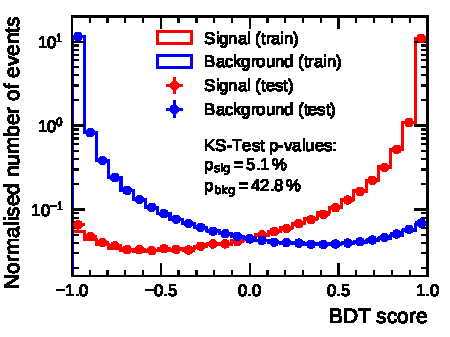
\includegraphics{./figures/bdt_perf/scores/grid_3p0327.pdf}
    \subcaption{BDT B}
  \end{subfigure}
  \caption[Distribution of the tau identification BDT score
  (3-prong)]{Distributions of the 3-prong tau identification BDT score for the
    training and testing sample for signal and background candidates.}
  \label{fig:bdt_ks5_scores}
\end{minipage}

\FloatBarrier
\subsection{Comparison of BDT A and BDT B}

\noindent
\begin{minipage}{\textwidth}
  \captionsetup{type=figure}
  \begin{subfigure}[t]{0.48\textwidth}
    \centering
    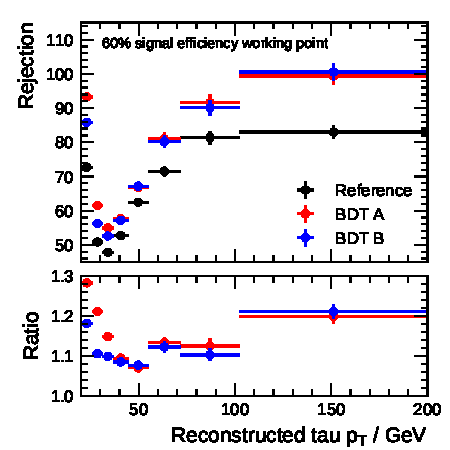
\includegraphics{./figures/bdt_perf/rejection/post_gridsearch_1p/rejection_tight.pdf}
    \subcaption{1-prong (tight)}
  \end{subfigure}\hfill
  \begin{subfigure}[t]{0.48\textwidth}
    \centering
    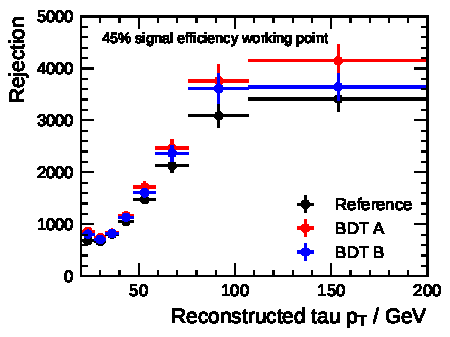
\includegraphics{./figures/bdt_perf/rejection/post_gridsearch_3p/rejection_tight.pdf}
    \subcaption{3-prong (tight)}
  \end{subfigure}
  \caption{Working points (BDT A).}
\end{minipage}

\FloatBarrier
\subsection{Recursive Feature Elimination}
\noindent
\begin{minipage}{\textwidth}
  \captionsetup{type=figure}
  \centering
  \begin{subfigure}[t]{0.33\textwidth}
    \centering
    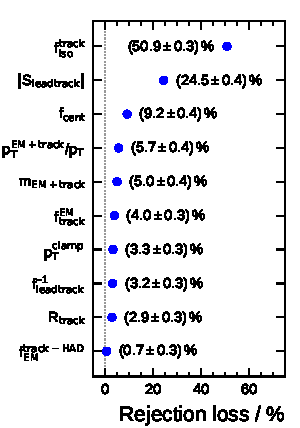
\includegraphics{./figures/bdt_perf/var_importance/1p_iter1.pdf}
    \subcaption{Iteration 1}
  \end{subfigure}
  \begin{subfigure}[t]{0.33\textwidth}
    \centering
    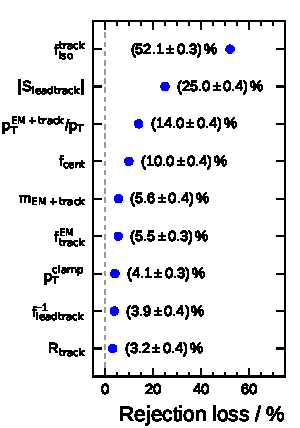
\includegraphics{./figures/bdt_perf/var_importance/1p_iter2.pdf}
    \subcaption{Iteration 2}
  \end{subfigure}
  \caption{Variable importance (1-prong). Averaged rejection loss over a
    gamma-tautau like dijet spectrum. Tight working point.}
  \label{fig:variable_importance_1p_app}
\end{minipage}

\noindent
\begin{minipage}{\textwidth}
  \captionsetup{type=figure}
  \centering
  \begin{subfigure}[t]{0.32\textwidth}
    \centering
    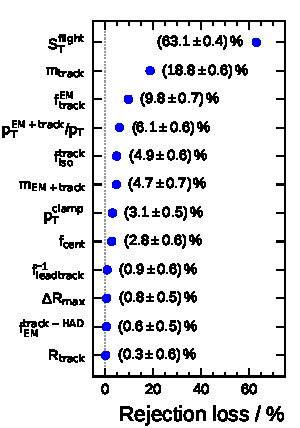
\includegraphics{./figures/bdt_perf/var_importance/3p_iter1.pdf}
    \subcaption{Iteration 1}
  \end{subfigure}
  \begin{subfigure}[t]{0.32\textwidth}
    \centering
    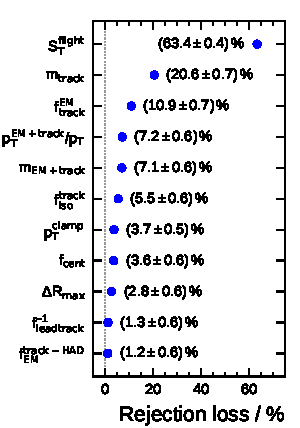
\includegraphics{./figures/bdt_perf/var_importance/3p_iter2.pdf}
    \subcaption{Iteration 2}
  \end{subfigure}
  \begin{subfigure}[t]{0.32\textwidth}
    \centering
    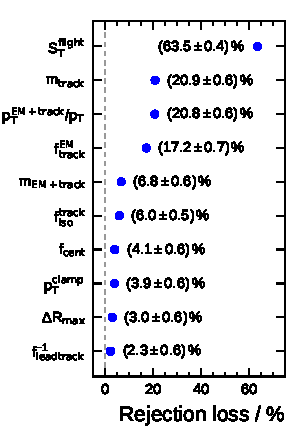
\includegraphics{./figures/bdt_perf/var_importance/3p_iter3.pdf}
    \subcaption{Iteration 3}
  \end{subfigure}

  \caption{Variable importance (3-prong). Averaged rejection loss over a
    gamma-tautau like dijet spectrum. Tight working point.}
  \label{fig:variable_importance_3p_app}
\end{minipage}

\FloatBarrier
\subsection{Tau Identification Performance Depending on the Initiating Parton}
\label{app:bdt_parton}

\noindent
\begin{minipage}{\textwidth}
  \captionsetup{type=figure}
  \centering
  \begin{subfigure}[t]{0.48\textwidth}
    \centering
    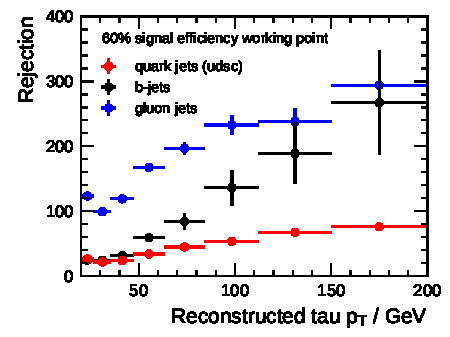
\includegraphics{./figures/bdt_perf/parton/truth_parton_1p.pdf}
    \subcaption{1-prong}
  \end{subfigure}\hfill
  \begin{subfigure}[t]{0.48\textwidth}
    \centering
    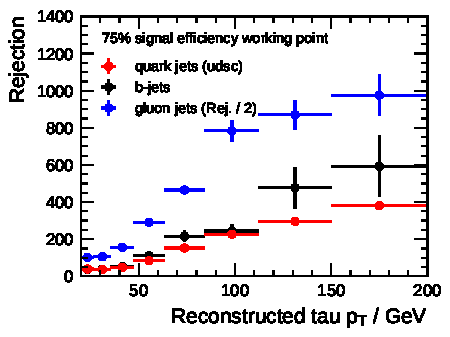
\includegraphics{./figures/bdt_perf/parton/truth_parton_3p.pdf}
    \subcaption{3-prong}
  \end{subfigure}
  \caption[Background rejection of the BDT depending on the initiating
  parton]{Background rejection of the optimised BDT for tau identification
    depending on the parton that initiated the jet.}
\end{minipage}

\clearpage
\subsection{Medium and Loose Working Points of the Optimised BDT}
\label{app:bdt_working_point_rejection}
\noindent
\begin{minipage}{\textwidth}
  \captionsetup{type=figure}
  \begin{subfigure}{0.48\textwidth}
    \centering
    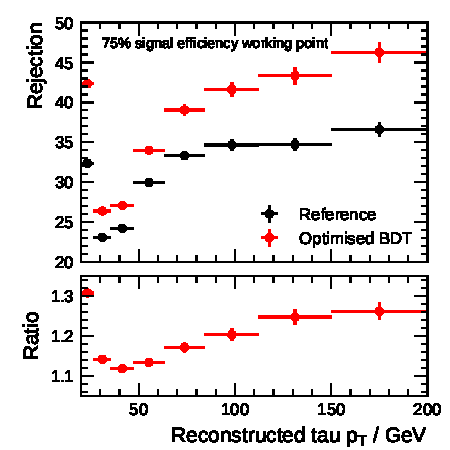
\includegraphics{./figures/bdt_perf/post_optimisation/rejection_medium_1p.pdf}
    \subcaption{medium}
  \end{subfigure}\hfill
  \begin{subfigure}{0.48\textwidth}
    \centering
    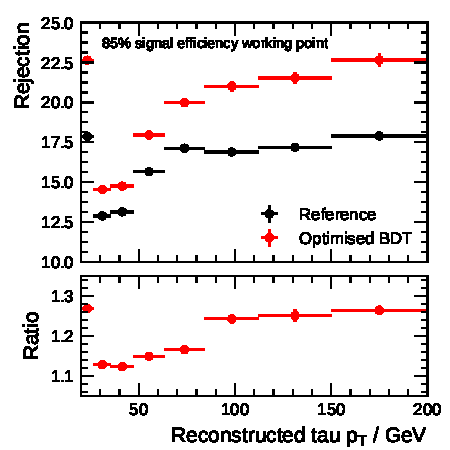
\includegraphics{./figures/bdt_perf/post_optimisation/rejection_loose_1p.pdf}
    \subcaption{loose}
  \end{subfigure}
  \caption[Background rejection of the 1-prong medium and loose working points
  in bins of \tauhadvis~\pt for the BDT-based identification]{Background
    rejection of the 1-prong medium and loose working points in bins of
    \tauhadvis~\pt.}
\end{minipage}

\noindent
\begin{minipage}{\textwidth}
  \captionsetup{type=figure}
  \begin{subfigure}{0.48\textwidth}
    \centering
    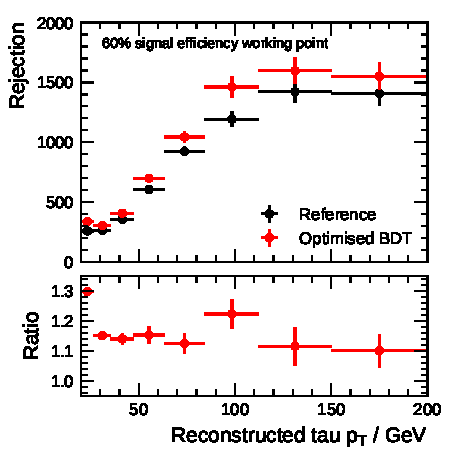
\includegraphics{./figures/bdt_perf/post_optimisation/rejection_medium_3p.pdf}
    \subcaption{medium}
  \end{subfigure}\hfill
  \begin{subfigure}{0.48\textwidth}
    \centering
    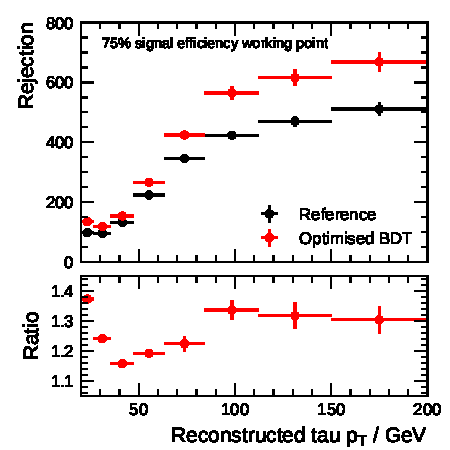
\includegraphics{./figures/bdt_perf/post_optimisation/rejection_loose_3p.pdf}
    \subcaption{loose}
  \end{subfigure}
  \caption[Background rejection of the 3-prong medium and loose working points
  in bins of \tauhadvis~\pt for the BDT-based identification]{Background
    rejection of the 3-prong medium and loose working points in bins of
    \tauhadvis~\pt.}
\end{minipage}

\noindent
\begin{minipage}{\textwidth}
  \captionsetup{type=figure}
  \begin{subfigure}{0.48\textwidth}
    \centering
    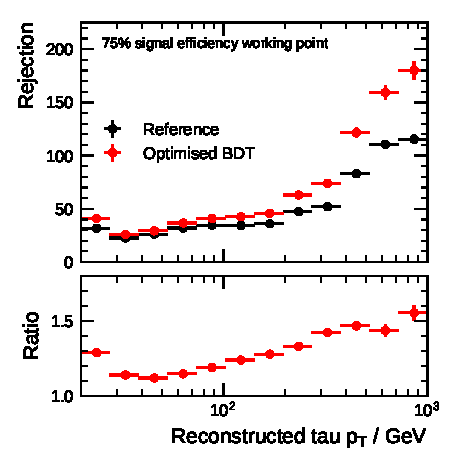
\includegraphics{./figures/bdt_perf/post_optimisation/1p_highpt/rejection_medium_ratio_highpt.pdf}
    \subcaption{medium}
  \end{subfigure}\hfill
  \begin{subfigure}{0.48\textwidth}
    \centering
    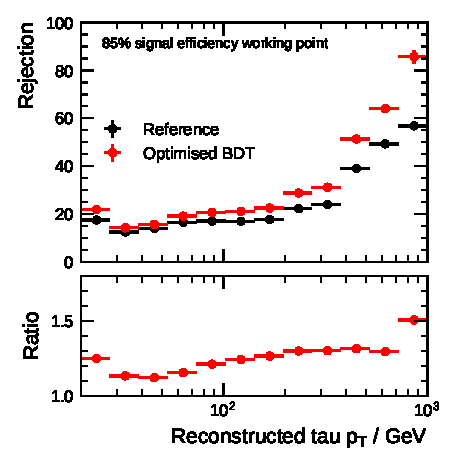
\includegraphics{./figures/bdt_perf/post_optimisation/1p_highpt/rejection_loose_ratio_highpt.pdf}
    \subcaption{loose}
  \end{subfigure}
  \caption{1-prong high-pt}
\end{minipage}

\noindent
\begin{minipage}{\textwidth}
  \centering
  \captionsetup{type=figure}
  \begin{subfigure}{0.48\textwidth}
    \centering
    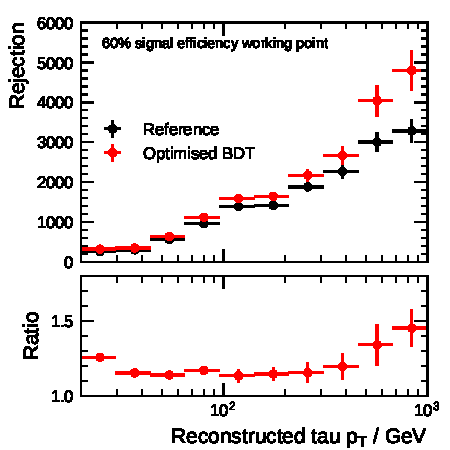
\includegraphics{./figures/bdt_perf/post_optimisation/3p_highpt/rejection_medium_ratio_highpt.pdf}
    \subcaption{medium}
  \end{subfigure}\hfill
  \begin{subfigure}{0.48\textwidth}
    \centering
    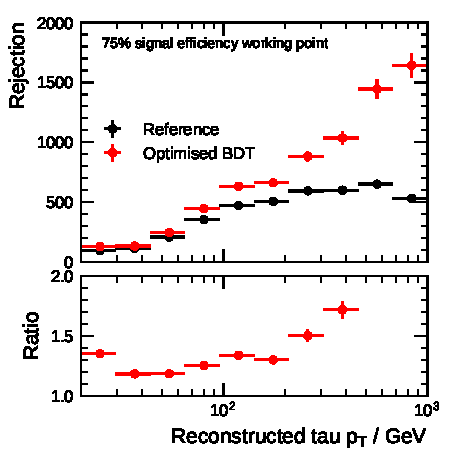
\includegraphics{./figures/bdt_perf/post_optimisation/3p_highpt/rejection_loose_ratio_highpt.pdf}
    \subcaption{loose}
  \end{subfigure}
  \caption{3-prong high-pt}
\end{minipage}


\clearpage
\section{Tau Identification using Recurrent Neural Networks}
\label{app:rnn}

\subsection{Number of Tracks and Clusters Associated with 3-prong Tau
  Candidates}

\noindent
\begin{minipage}{\textwidth}
  \captionsetup{type=figure}
  \begin{subfigure}[t]{0.48\textwidth}
    \centering
    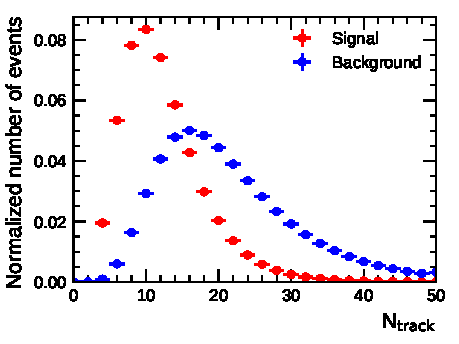
\includegraphics{./figures/rnn/ntrk_3p.pdf}
    \subcaption{Tracks}
  \end{subfigure}\hfill
  \begin{subfigure}[t]{0.48\textwidth}
    \centering
    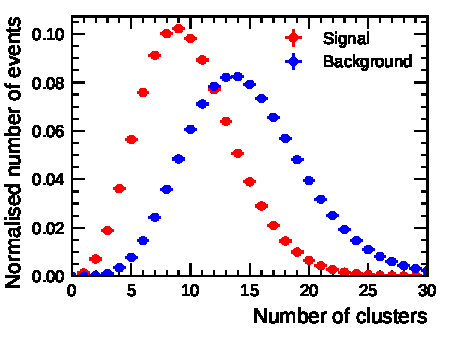
\includegraphics{./figures/rnn/ncls_3p.pdf}
    \subcaption{Clusters}
  \end{subfigure}
  \caption{Number of tracks and clusters associated with 3-prong \tauhadvis
    candidates.}
\end{minipage}

\subsection{Correlation of Estimated Signal Probability and Distance of Tracks
  to the Jet Axis}
\label{app:corr_dr}

\noindent
\begin{minipage}{\textwidth}
  \captionsetup{type=figure}
  \centering
  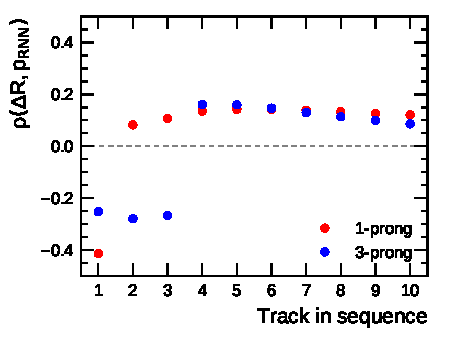
\includegraphics{./figures/rnn/track/dR_corr.pdf}
  \caption{Linear correlation coefficient between the track distance~$\Delta R$
    to the jet axis and the signal probability~$p_\text{RNN}$ estimated by the
    model from Section~\ref{sec:rnn_tracks}. The coefficient is determined on
    the testing sample combining signal and background candidates with equal
    total weight.}
\end{minipage}

\subsection{Combined RNN Working Points}
\label{app:rnn_wp}

\noindent
\begin{minipage}{\textwidth}
  \captionsetup{type=figure}
  \begin{subfigure}[t]{0.48\textwidth}
    \centering
    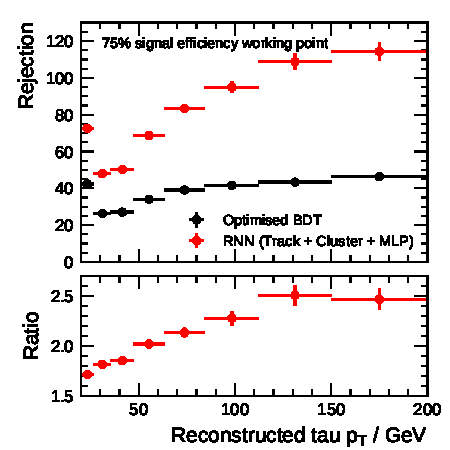
\includegraphics{./figures/rnn/combined/rnn_medium_1p.pdf}
    \subcaption{loose}
  \end{subfigure}\hfill
  \begin{subfigure}[t]{0.48\textwidth}
    \centering
    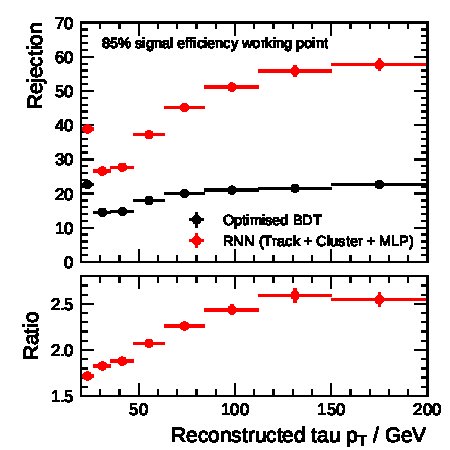
\includegraphics{./figures/rnn/combined/rnn_loose_1p.pdf}
    \subcaption{medium}
  \end{subfigure}
  \caption{Background rejection at the medium working point as a function of the
    reconstructed tau $p_\text{T}$ at tau energy scale for the BDT- and
    RNN-based identification.}
\end{minipage}

\vfill

\noindent
\begin{minipage}{\textwidth}
  \captionsetup{type=figure}
  \begin{subfigure}[t]{0.48\textwidth}
    \centering
    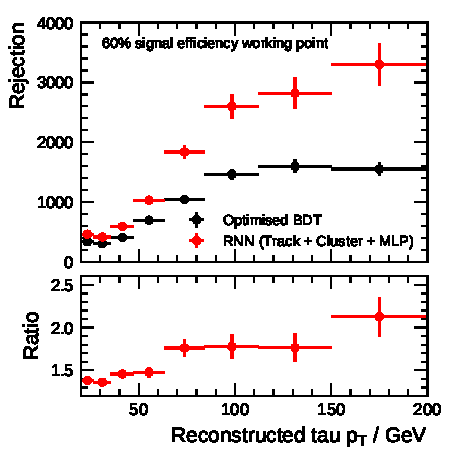
\includegraphics{./figures/rnn/combined/rnn_medium_3p.pdf}
    \subcaption{loose}
  \end{subfigure}\hfill
  \begin{subfigure}[t]{0.48\textwidth}
    \centering
    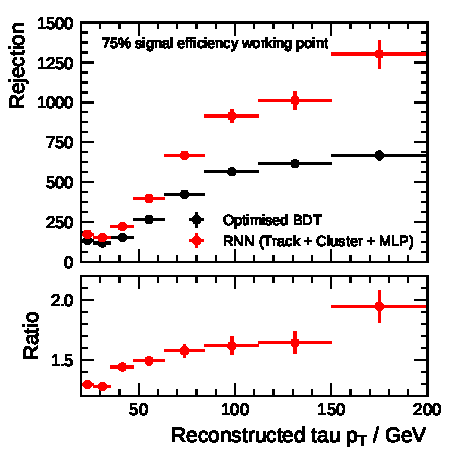
\includegraphics{./figures/rnn/combined/rnn_loose_3p.pdf}
    \subcaption{medium}
  \end{subfigure}
  \caption{Background rejection at the loose working point as a function of the
    reconstructed tau $p_\text{T}$ at tau energy scale for the BDT- and
    RNN-based identification.}
\end{minipage}

\clearpage
\section{Decay Mode Classification using Recurrent Neural Networks}
\label{app:decay_mode}

\subsection{Estimated Mode Probabilities: Baseline Model}
\label{app:baseline_probabilities}

\noindent
\begin{minipage}{\textwidth}
  \captionsetup{type=figure}
  \begin{subfigure}{0.48\textwidth}
    \centering
    \includegraphics{./figures/decay_mode_classification/mode_proba_baseline_ptcut_1_5/proba_1p0n.pdf}
  \end{subfigure}\hfill
  \begin{subfigure}{0.48\textwidth}
    \centering
    \includegraphics{./figures/decay_mode_classification/mode_proba_baseline_ptcut_1_5/proba_1p1n.pdf}
  \end{subfigure}
  \begin{subfigure}{0.48\textwidth}
    \centering
    \includegraphics{./figures/decay_mode_classification/mode_proba_baseline_ptcut_1_5/proba_1pXn.pdf}
  \end{subfigure}\hfill
  \begin{subfigure}{0.48\textwidth}
    \centering
    \includegraphics{./figures/decay_mode_classification/mode_proba_baseline_ptcut_1_5/proba_3p0n.pdf}
  \end{subfigure}
  \begin{subfigure}{0.48\textwidth}
    \centering
    \includegraphics{./figures/decay_mode_classification/mode_proba_baseline_ptcut_1_5/proba_3pXn.pdf}
  \end{subfigure}%

  \caption{Multi-class probabilities for the Baseline RNN}
  \label{fig:rnn_multiclass_proba_baseline}
\end{minipage}

\clearpage
\subsection{Estimated Mode Probabilities: Extended Model}
\label{app:combined_probabilities}

\noindent
\begin{minipage}{\textwidth}
  \captionsetup{type=figure}
  \begin{subfigure}{0.48\textwidth}
    \centering
    \includegraphics{./figures/decay_mode_classification/combined_proba/proba_1p0n.pdf}
  \end{subfigure}\hfill
  \begin{subfigure}{0.48\textwidth}
    \centering
    \includegraphics{./figures/decay_mode_classification/combined_proba/proba_1p1n.pdf}
  \end{subfigure}
  \begin{subfigure}{0.48\textwidth}
    \centering
    \includegraphics{./figures/decay_mode_classification/combined_proba/proba_1pXn.pdf}
  \end{subfigure}\hfill
  \begin{subfigure}{0.48\textwidth}
    \centering
    \includegraphics{./figures/decay_mode_classification/combined_proba/proba_3p0n.pdf}
  \end{subfigure}
  \begin{subfigure}{0.48\textwidth}
    \centering
    \includegraphics{./figures/decay_mode_classification/combined_proba/proba_3pXn.pdf}
  \end{subfigure}%

  \caption{Multi-class probabilities for the Combined RNN}
  \label{fig:rnn_multiclass_proba_combined}
\end{minipage}

\clearpage
\subsection{Migration and Purity Matrices when Including Additional Information}
\label{sec:app_decay_mode_exp}

This section summarises the migration and purity matrices of the different
classification setups described in Section~\ref{sec:add_info}.

\vfill

\noindent
\begin{minipage}{\textwidth}
  \captionsetup{type=figure}
  \begin{subfigure}[t]{0.48\textwidth}
    \centering
    \includegraphics{./figures/decay_mode_classification/experiments/mig_mat_conversions.pdf}
  \end{subfigure}\hfill
  \begin{subfigure}[t]{0.48\textwidth}
    \centering
    \includegraphics{./figures/decay_mode_classification/experiments/comp_mat_conversions.pdf}
  \end{subfigure}
  \caption{Migration and purity matrices of the baseline model extended with
    conversion tracks.}
\end{minipage}

\vfill

\noindent
\begin{minipage}{\textwidth}
  \captionsetup{type=figure}
  \begin{subfigure}[t]{0.48\textwidth}
    \centering
    \includegraphics{./figures/decay_mode_classification/experiments/mig_mat_shots.pdf}
  \end{subfigure}\hfill
  \begin{subfigure}[t]{0.48\textwidth}
    \centering
    \includegraphics{./figures/decay_mode_classification/experiments/comp_mat_shots.pdf}
  \end{subfigure}
  \caption{Migration and purity matrices of the baseline model extended with
    shots.}
\end{minipage}

\vfill

\noindent
\begin{minipage}{\textwidth}
  \captionsetup{type=figure}
  \begin{subfigure}[t]{0.48\textwidth}
    \centering
    \includegraphics{./figures/decay_mode_classification/experiments/mig_mat_moments.pdf}
  \end{subfigure}\hfill
  \begin{subfigure}[t]{0.48\textwidth}
    \centering
    \includegraphics{./figures/decay_mode_classification/experiments/comp_mat_moments.pdf}
  \end{subfigure}
  \caption{Migration and purity matrices of the baseline model extended with
    additional neutral PFO cluster properties.}
\end{minipage}

\clearpage
\subsection{Requiring Consistency with the Number of Reconstructed Tracks}
\label{app:mode_classification_track_constraint}

\noindent
\begin{minipage}{\textwidth}
  \captionsetup{type=figure}
  \begin{subfigure}{0.48\textwidth}
    \centering
    \includegraphics{./figures/decay_mode_classification/combined_sub_e_moments_shots_conv_ptcut_1_5/mig_mat.pdf}
    \subcaption{Extended model without track constraint}
  \end{subfigure}\hfill
  \begin{subfigure}{0.48\textwidth}
    \centering
    \includegraphics{./figures/decay_mode_classification/combined_sub_e_moments_shots_conv_ptcut_1_5/mig_mat_use_ntracks.pdf}
    \subcaption{Extended model with track constraint}
  \end{subfigure}
  \caption{Migration matrix for the extended model including conversion, shot
    and additional cluster information. The model is constrained by setting
    estimated mode probabilities to zero for modes not consistent with the
    number of reconstructed tracks.}
\end{minipage}

\subsection{Classification Performance after Medium Tau Identification}

\noindent
\begin{minipage}{\textwidth}
  \captionsetup{type=figure}
  \begin{subfigure}{0.48\textwidth}
    \centering
    \includegraphics{./figures/decay_mode_classification/combined_sub_e_moments_shots_conv_ptcut_1_5/mig_mat_med_id.pdf}
  \end{subfigure}\hfill
  \begin{subfigure}{0.48\textwidth}
    \centering
    \includegraphics{./figures/decay_mode_classification/combined_sub_e_moments_shots_conv_ptcut_1_5/comp_mat_med_id.pdf}
  \end{subfigure}
  \caption{Migration and purity matrices for the extended model after applying
    medium tau identification (BDT-based).}
  \label{fig:decay_mode_combined_med_id}
\end{minipage}

\clearpage
\subsection{Classification Performance at High Transverse Momenta}
\label{sec:combined_high_pt_migration}

\begin{figure}[htb]
    \begin{subfigure}{0.48\textwidth}
    \centering
    \includegraphics{./figures/decay_mode_classification/highpt/mig_mat_pt_less_100.pdf}
    \subcaption{Migration matrix. $p_\text{T} < \SI{100}{\giga\electronvolt}$}
  \end{subfigure}\hfill
  \begin{subfigure}{0.48\textwidth}
    \centering
    \includegraphics{./figures/decay_mode_classification/highpt/comp_mat_pt_less_100.pdf}
    \subcaption{Purity matrix. $p_\text{T} < \SI{100}{\giga\electronvolt}$}
  \end{subfigure}
  \begin{subfigure}{0.48\textwidth}
    \centering
    \includegraphics{./figures/decay_mode_classification/highpt/mig_mat_pt_geq_100.pdf}
    \subcaption{Migration matrix. $p_\text{T} > \SI{100}{\giga\electronvolt}$}
  \end{subfigure}\hfill
  \begin{subfigure}{0.48\textwidth}
    \centering
    \includegraphics{./figures/decay_mode_classification/highpt/comp_mat_geq_100.pdf}
    \subcaption{Purity matrix. $p_\text{T} > \SI{100}{\giga\electronvolt}$}
  \end{subfigure}
  \caption{highpt}
  \label{fig:highpt_matrices}
\end{figure}

%%% Local Variables:
%%% mode: latex
%%% TeX-master: "mythesis"
%%% End:
